\section{Types and evaluation metrics}
The following  are the output types described in the official BioASQ evaluation documentation \cite{145}:
\subsubsection{Snippets}
\begin{displayquote}
$s_{i,1} , s_{i,2}, s_{i,3}, \hdots$ from the returned articles. Again, the list should be ordered by decreasing confidence. A single snippet list will be returned per question and participant, and the list may contain any number (or no) snippets from any of the returned articles $d_{i,1}, d_{i,2}, d_{i,3}, \hdots, d_{i,k}$. Each snippet will be represented by the unique identifier of the article it comes from and the offsets (character positions in the article) of the snippet’s beginning and end (offsets of the first and last characters).
\end{displayquote}
\textbf{Example:} Here the JSON array \verb|snippets| corresponds to document snippets.  
\small
\begin{verbatim}
"body": "What is the role of PrnP in mad cow disease?", 
      "type": "factoid", 
      "id": "160",
      "snippets" : [ 
                   {
                       "document": "http://www.ncbi.nlm.nih.gov/pubmed/23217568", 
                       "beginSection": "sections.0", 
                       "endSection": "sections.0", 
       	               "offsetInBeginSection": 591, 
                       "offsetInEndSection": 678, 
                       "text": "Our results show a high prevalence of RA ..."
                   },
	                 ...
	                 {
                       "beginSection": "sections.0", 
                       "document": "http://www.ncbi.nlm.nih.gov/pubmed/23217568", 
                       "endSection": "sections.0", 
                       "offsetInBeginSection": 1140, 
                       "offsetInEndSection": 1394, 
                       "text": "RA in LAC women is not only more common but presents..."
	                 }]
\end{verbatim}
\normalsize
Note that for each phase you will return a list of $k$ items in order of decreasing confidence (where $k \leq 100$). See the evaluation section below for how these will be evaluated. 
  
\subsection{Evaluation}
Please refer to table \ref{fig:eval} to see the evaluation used for each type.
\begin{figure}[h!]
\begin{tabular}{|c|c|c|}
\hline
	\textbf{Retrieved items} & \textbf{Unordered retrieval measures} & \textbf{Ordered retrieval measures}\\ \hline
	snippets & mean percision, recall, F-measure & MAP,\textbf{GMAP}\\ \hline
\end{tabular}
\label{fig:eval}
\caption{Evaluation metrics}
\end{figure}

Also, please review the definitions of the evaluation metrics. Note that the definitions for Precision and Recall for document snippets are slightly different than the metrics you used in M1:

\begin{itemize}
\item Precision and Recall:
\begin{comment}
\begin{align}
P &= \dfrac{TP}{TP + FP} \tag{where TP are true positives, and FP are false positives}\\
R &= \dfrac{TP}{TP + FN} \tag{where TP are true positives, and FN are false negatives}
\end{align}
\end{comment}

\begin{align}
P_{snip} &= \dfrac{|S \cap G|}{|S|}\\
R_{snip} &= \dfrac{|S \cap G|}{|G|}
\end{align}
Where $S$ is the set of all article-offset paris of all the characters in the snippet, and $G$ is the set of all the article-offset pairs of all the characters in the golden snippet. See \ref{fig:snippets} for an illustration of an article-offset pair in an article.

\begin{figure}
\centering
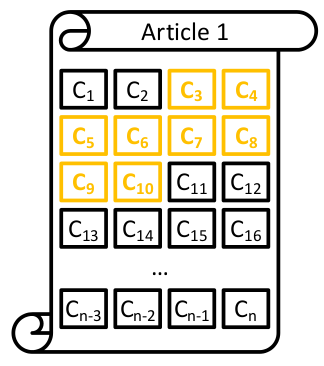
\includegraphics[scale=0.6]{bioqa/snippets.png}
\caption{An example of a golden snippet starting at offset 3 and ending at offset 10.}
\label{fig:snippets}
\end{figure}
\item F-measure:
\begin{align}
F = 2 \cdot \dfrac{P\cdot R}{P + R} \tag{Harmonic mean of Precision and Recall}
\end{align}
\item Average Precision (AP):
\begin{align}
AP &= \dfrac{\sum^{|L|}_{r=1} P(r) \cdot rel(r)}{L_R} \tag{see below}
\end{align} 
Where, for any given query $q_i$ and a golden set of items:
\begin{itemize}
\item $|L|$ is the total number of items.
\item $|L_R|$ is the number of relevant items. 
\item $P(r)$ is the precision for a list containing the first $r$ items.
\item $rel(r)$ is an indicator function for the existence of item $r$ in the golden set (i.e., it returns 1 if the $r$th item is relevant, and 0 otherwise).
\end{itemize}
\item Mean Average Precision (MAP):
\begin{align}
MAP &= \frac{1}{n} \sum^n_{i=1}AP_i  \tag{To get the average precision for list of queries $q_1, q_2, \dots, q_n$.}
\end{align}
\item Geometric Mean Average Precision (GMAP):
\begin{align}
GMAP &= \sqrt[n]{\prod^n_{i=1}(AP_i + \epsilon)} \tag{with some small $\epsilon$ for cases where $AP_i=0$}
\end{align}
GMAP is similar to MAP, only used to further penalize low performing queries.
\end{itemize}

\section{Archetype}
\subsection{Typesystem}
For this milestone, you are required to use the typesystem \verb|OAQATypes.xml| included in the archetype. Note however, you are only required to use the types defined in \ref{ref:mappings} and their supertype ancestry. You are of course welcome to extend the typesystem and/or use any other preexisting types. Most importantly. it is imperative that you use the inherited \verb|uri| and \verb|rank| attributes, as we will use them for evaluation.
\begin{figure}[h!]
\begin{longtable}{c|P{6cm}}
\textbf{BioASQ Type} & \textbf{UIMA Type}\\\hline
Result (supertype) &   \begin{itemize} \item \verb|edu.cmu.lti.oaqa.type.retrieval.SearchResult| \begin{itemize} \item \verb|uri| \item \verb|rank| \end{itemize} \end{itemize} \\\hline
Snippet & \begin{itemize} \item \verb|edu.cmu.lti.oaqa.type.retrieval.Passage| \begin{itemize} \item \verb|uri| (inherited) \item \verb|rank| (inherited) \end{itemize}  \end{itemize} \\\hline
\end{longtable}
\label{ref:mappings}
\caption{Typesystem Mapping}
\end{figure}
\subsection{Web Services}
\label{subsec:WebServices}
Unlike in M1, there is no client for M2. To access the web service below you will simply query \url{http://metal.lti.cs.cmu.edu:30002/pmc/PMID} with the PMID you retrieved from the previous services.
\begin{itemize}
\item Full Document Sources: a service for accessing the \emph{PMC} full text articles, with the same input parameters and output parameters as aforementioned, with the only difference being that the articles returned contain in addtion the full text.
\end{itemize}
\subsection{Data}
In the archetype you will also find \verb|BioASQ-SampleData1B.json| containing an annotated version of the 29 sample questions shown in M0. We also provide you with a convenience class \verb|JsonCollectionReaderHelper.java| to read from JSON format. 


